\documentclass[12pt]{article}
\usepackage{amssymb}
\usepackage[UTF8]{ctex}
\usepackage{geometry}
\usepackage{units}
\usepackage{pifont}
\geometry{
	a4paper,
	total={150mm,237mm},
	left=30mm,
	top=27mm,
	}
\usepackage{amsmath}
\usepackage{enumerate}
\usepackage{lipsum}
\usepackage{graphicx}
\usepackage{hyperref}
\usepackage{indentfirst}
\usepackage[graphicx]{realboxes}
\usepackage{booktabs}
\usepackage{cases}
\usepackage{subfig}  
\usepackage{float}
\usepackage{xcolor}


\setlength{\parindent}{2em}
\title{Lab0}
\author{姓名:陈锐林,学号:21307130148}
\date{\today}

\begin{document}
\maketitle
\begin{large}
    \noindent 一、log\_stdout.c:\\
\end{large}
1.分析:\\
\hspace*{2em}这题要求实现read\_stdin和log\_stdout两个函数,具体要求为,根据输入值i,将标准输出重定向到i.log;对于标准输入,先读入到buf,再重定向到i.log。\\
2.实现:\\
\hspace*{2em}实现:实现log\_stdout,分为两个步骤,一是根据输入得到i的值,这里将i的每一位转为char;二是关闭标准输出,用open函数将fd(1)重定向到i.log。实现read\_stdin,只要一位位读入到预先设置好的buf缓冲区,最后直接printf就到i.log了。
\begin{figure*}[!h]
    \centering
    \subfloat[read\_stdin]{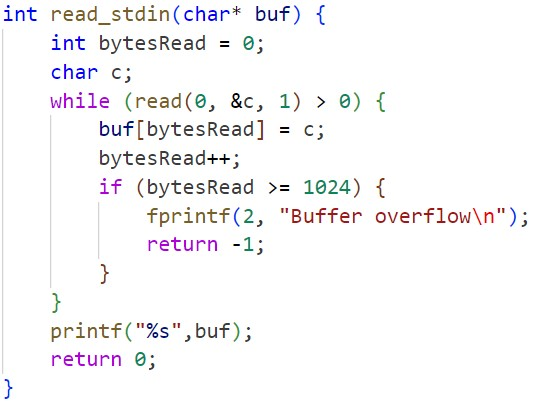
\includegraphics[width=5cm,height=5cm]{lab0-1.jpg} \label{X}}
    \hfill
    \subfloat[log\_stdout]{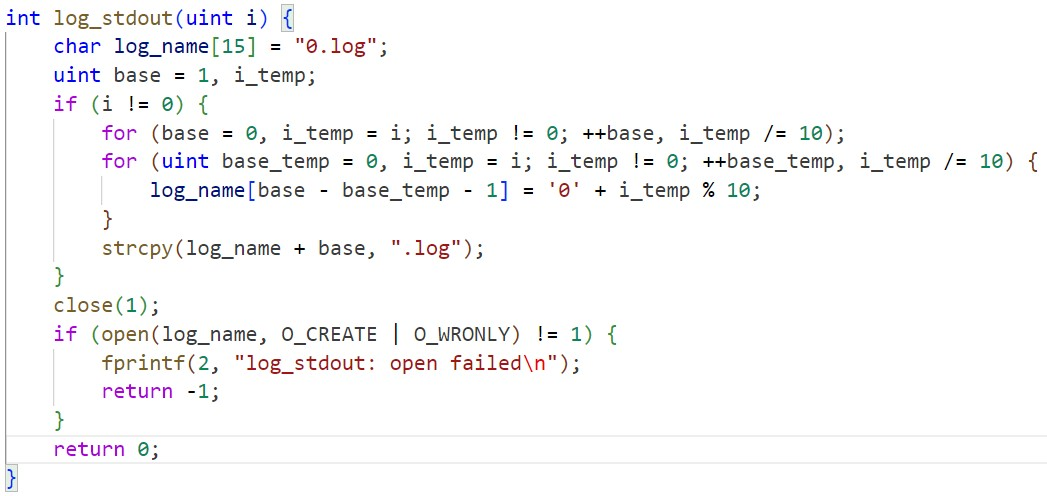
\includegraphics[width=8cm,height=5cm]{lab0-2.jpg} \label{Y}}
\end{figure*}\\
3.运行效果:
\begin{figure}[h]
    \centering
    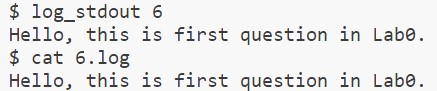
\includegraphics[width=9cm,height=3cm]{lab0-3.jpg}
\end{figure}
\newpage
\begin{large}
    \noindent 二、composites.c:\\
\end{large}
1.分析:\\
\hspace*{2em}这题要求补全composites和sub\_progress两个函数。(这里对sub\_progress进行了略微的修改)。sub\_progress实现思路为,每次取出输入的第一个数(已确保是素数),将其输出;然后遍历并去除其倍数,利用管道,不断将未考察的数(考察:即已被找到的素数和其倍数)作为当前父进程的输出和子进程的输入。\\
2.实现:\\
\hspace*{2em}在这里,通过write和read完成对管道的读写,调用log\_stdout作重定向输出;每次都输入一个-1在数组的末尾,作为哨兵,如果只剩-1就退出程序。为了便于实现(确保输出结果的工整),让子进程先sleep一会再继续执行。composites函数完成数组的初始化及导入和第一次子进程。需注意要等待子进程完成并且及时关闭不用的管道。
\begin{figure*}[!h]
    \centering
    \subfloat[sub\_progress]{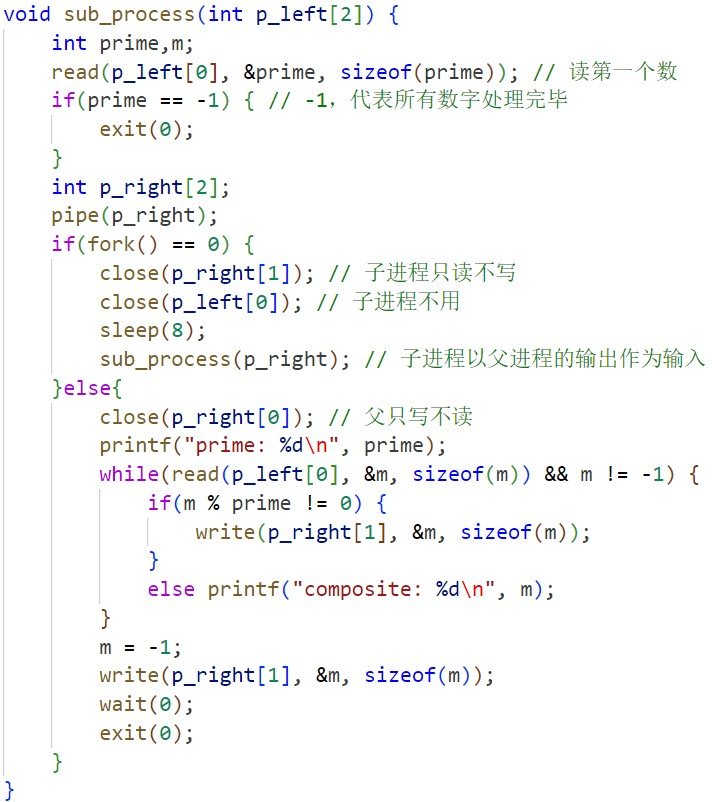
\includegraphics[width=7cm,height=7cm]{lab0-4.jpg} \label{X}}
    \hfill
    \subfloat[composites]{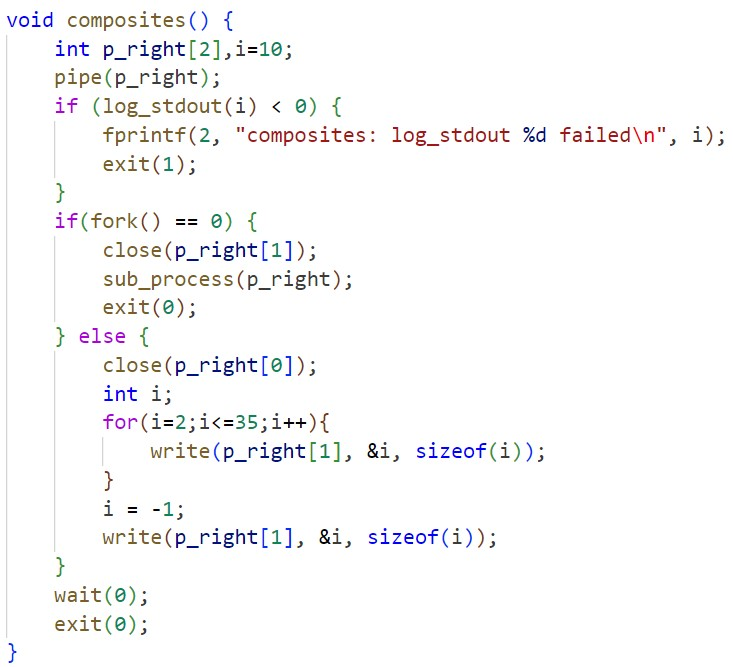
\includegraphics[width=7cm,height=7cm]{lab0-5.jpg} \label{Y}}
\end{figure*}\\
3.运行效果:顺序为从左往右,最后几个素数没截取
\begin{figure*}[!h]
    \centering
    \subfloat[part1]{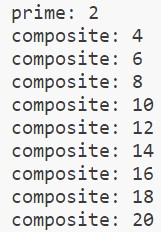
\includegraphics[width=2.5cm,height=4.5cm]{lab0-6.jpg} \label{X}}
    \hfill
    \subfloat[part2]{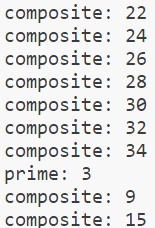
\includegraphics[width=2.5cm,height=4.5cm]{lab0-7.jpg} \label{Y}}
    \hfill
    \subfloat[part3]{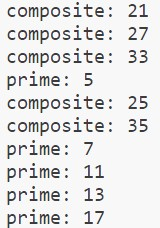
\includegraphics[width=2.5cm,height=4.5cm]{lab0-8.jpg} \label{Y}}
\end{figure*}
\newpage
\begin{large}
    \noindent 三、xargs.c:\\
\end{large}
1.分析:\\
\hspace*{2em}题目要求从标准输入读取多个参数并且执行,大致思路为利用fork出的子进程调用exec即可。\\
2.实现:\\
\hspace*{2em}由hint可知要注意换行符,以及可以直接调用的MAXARG。具体实现时,先保存argv中的参数(注意索引),之后从标准输入小心地每次读入一个字符,碰到换行符了要特殊处理,fork出子进程执行参数;否则就正常后移指针,当这个读入循环结束时,该函数的目标也达到了。
\begin{figure}[h]
    \centering
    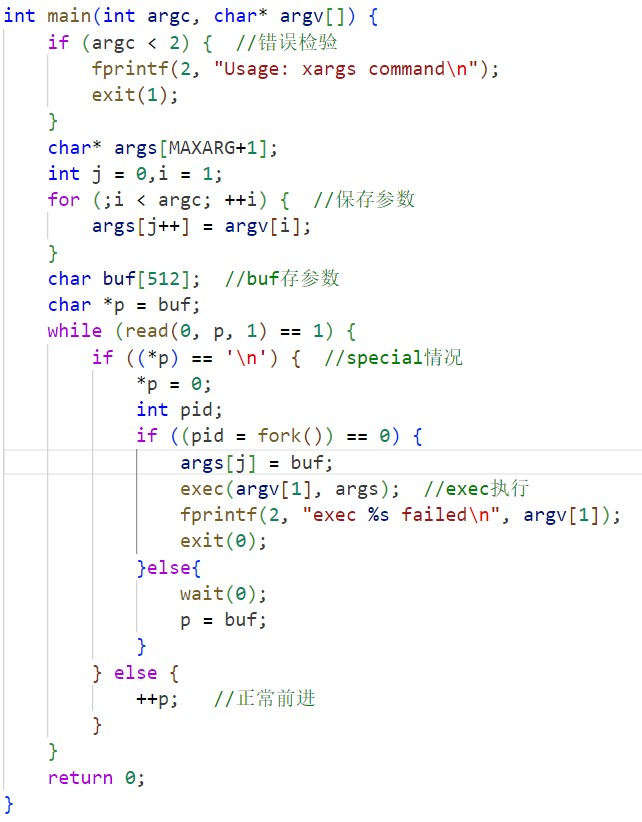
\includegraphics[height=10cm,width=11cm]{lab0-11.jpg}
\end{figure}\\
3.运行效果:取两个例子验证
\begin{figure*}[!h]
    \centering
    \subfloat[example1]{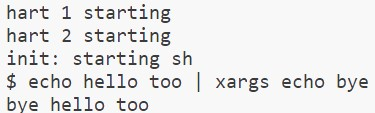
\includegraphics[width=5cm,height=2cm]{lab0-9.jpg}}
    \hfill
    \subfloat[example2]{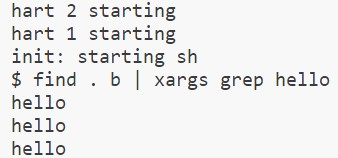
\includegraphics[width=5cm,height=2cm]{lab0-10.jpg}}
\end{figure*}
\end{document}